\documentclass[11pt,a4paper]{article}
\usepackage[T1]{fontenc}
\usepackage[utf8]{inputenc}
\usepackage[french]{babel}
\usepackage{lmodern}
\usepackage[margin=2.2cm]{geometry}
\usepackage{graphicx}
\usepackage{booktabs}
\usepackage{caption}
\usepackage{float}
\usepackage{tikz}
\usetikzlibrary{arrows.meta,positioning}
\usepackage[hidelinks]{hyperref}
\captionsetup{font=small,labelfont=bf}

\newcommand{\valnpoints}{367}
\newcommand{\valnunsure}{19}
\newcommand{\valnuniform}{184}
\newcommand{\valacc}{0{,}80}
\newcommand{\valacclo}{0{,}74}
\newcommand{\valacchi}{0{,}85}
\newcommand{\valaccstring}{0{,}68}
\newcommand{\valcolourok}{0{,}91}
\newcommand{\valncolour}{78}
\newcommand{\valmissed}{0{,}15}
\newcommand{\vallostshadow}{0{,}03}


\title{Segmentation des couleurs des nids de diamants mandarins\\[2pt]
\large Évolution des versions et validation indépendante}
\author{Projet \emph{Nest weave quantif}}
\date{19 novembre 2026}

\begin{document}
\maketitle

\begin{abstract}
Les nids sont construits avec des ficelles de quatre couleurs fournies successivement
(orange, jaune, blanc, puis rouge à la ponte). Toutes les mesures de mélange et de stratification
reposent sur une carte qui attribue une classe à chaque pixel de la photo. Ce document montre
comment cette carte a évolué entre les versions v3, v4 et v5b, sur les images qui ont servi à
l'annotation, et ce que vaut la version actuelle (v5b) face à une annotation humaine
à l'aveugle de \valnpoints{} points : exactitude globale \valacc{} [\valacclo--\valacchi],
et \valcolourok{} lorsque le modèle et l'annotatrice voient tous deux une ficelle de couleur.
\end{abstract}

\section{Données et méthode}

\paragraph{Images.} 32 photos de 8 nids et 10 séances de prise de vue (une à cinq vues : dessus,
face, gauche, droite, entrée), prises dans une boîte à lumière avec une mire. 8 photos (dossier
\texttt{data}) ont servi au développement initial ; 24 autres (dossier \texttt{all\_views}, archivé
le 01/11, qui contient aussi les 4 vues du 207) ont été ajoutées après la version v3.

\paragraph{Annotations d'entraînement.} Il n'existe pas d'images annotées au pixel près.
Le classifieur est entraîné sur environ 60 rectangles tracés à l'œil sur les photos, chacun associé à
une classe ; à l'intérieur d'un rectangle, seuls les pixels compatibles en couleur avec la classe sont
retenus (filtre de teinte et de saturation). Des « exemples négatifs » sans rectangle désignent
aussi, sur des nids sans ficelle blanche, les pixels blanchâtres comme du fond.

\paragraph{Chaîne de traitement.} La figure~\ref{fig:pipeline} résume les étapes.
L'étage A décide si un pixel est de la ficelle à partir de son voisinage (descripteurs multi-échelles
jusqu'à $\sigma = 8$~px, à demi-résolution) ; l'étage B attribue la couleur aux seuls pixels de ficelle,
à partir de descripteurs quasi ponctuels. Un pixel de ficelle nettement plus sombre que la luminance
typique de sa couleur devient « trou / ombre ». Enfin, un nettoyage par continuité (S2.4) retire les
îlots qu'aucun brin n'explique et comble les petits trous dans l'axe des brins.

\begin{figure}[H]
\centering
\begin{tikzpicture}[
  node distance=4mm,
  box/.style={draw=black!60, rounded corners=2pt, fill=black!4, align=center, font=\small,
              minimum height=10mm, text width=21mm},
  arr/.style={-{Stealth[length=2mm]}, black!70}]
\node[box] (p) {photo\\(balance des blancs)};
\node[box, right=of p] (a) {étage A\\ficelle / fond / autre};
\node[box, right=of a] (b) {étage B\\couleur};
\node[box, right=of b] (s) {ombre\\(luminance)};
\node[box, right=of s] (c) {S2.4\\continuité};
\draw[arr] (p) -- (a); \draw[arr] (a) -- (b); \draw[arr] (b) -- (s); \draw[arr] (s) -- (c);
\end{tikzpicture}
\caption{Chaîne de segmentation. Les étages A et B sont des forêts aléatoires entraînées sur les
rectangles annotés.}
\label{fig:pipeline}
\end{figure}

\section{Les versions}

Les versions v1 et v2 (un seul classifieur, puis deux étages sans classe d'ombre) n'ont pas été
archivées ; la comparaison commence donc à v3. Le tableau~\ref{tab:versions} résume ce qui change.

\begin{table}[H]
\centering\small
\begin{tabular}{l p{6.2cm} p{6.0cm}}
\toprule
version & changement & problème corrigé \\
\midrule
v3 & deux étages, balance des blancs, classe « trou / ombre », nids sans blanc en exemples
négatifs, rectangles sur la boîte filtrés par couleur &
fond vu à travers le nid compté comme du blanc ; brins devant la boîte classés « support » \\
v4 & nettoyage par continuité (S2.4) ; exemples « support » sur la bande sombre du contreplaqué &
mouchetures, liserés d'un pixel ; bande de bois classée orange (206) \\
v5b & exemples négatifs sur des nids jaunes sans blanc (109, 102 du 14/04), plafonnés à 3\,000 px
par image & liseré et trous « blancs » sur les nids jaunes \\
\bottomrule
\end{tabular}
\caption{Versions comparées. v5b est la segmentation de travail actuelle.}
\label{tab:versions}
\end{table}

\section{Vues d'ensemble}

\begin{figure}[H]
\centering
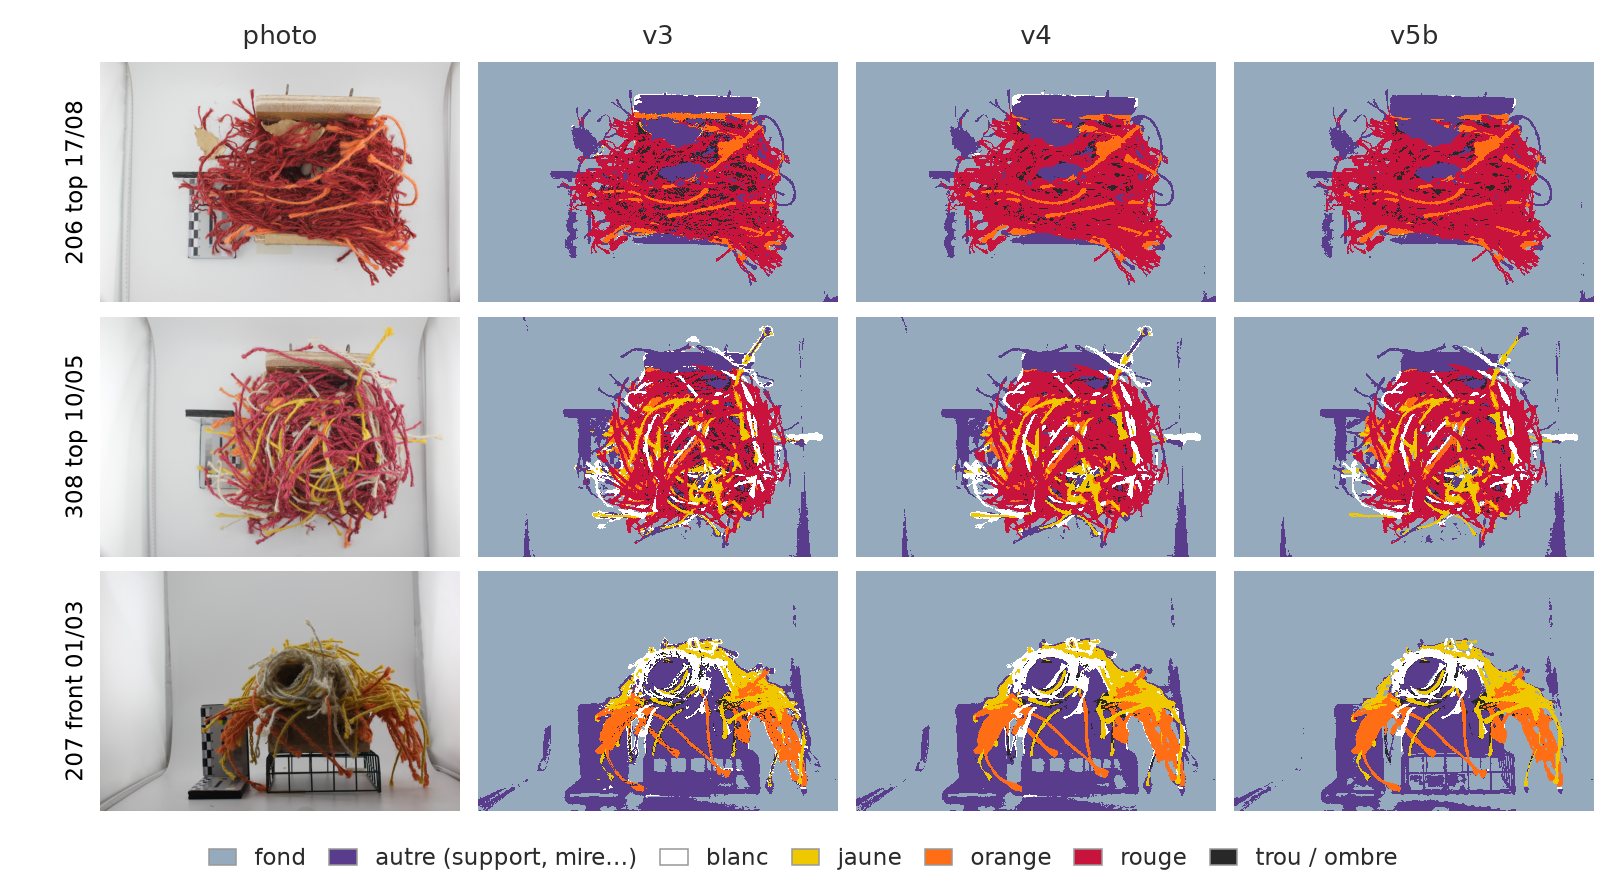
\includegraphics[width=\textwidth]{figs/overview_data.png}
\caption{Images du développement initial, trois versions. Les différences d'ensemble sont faibles :
elles se concentrent sur les bords des brins, les petits îlots et le blanc
(voir les zooms de la figure~\ref{fig:zooms}).}
\label{fig:overview-data}
\end{figure}

\begin{figure}[H]
\centering
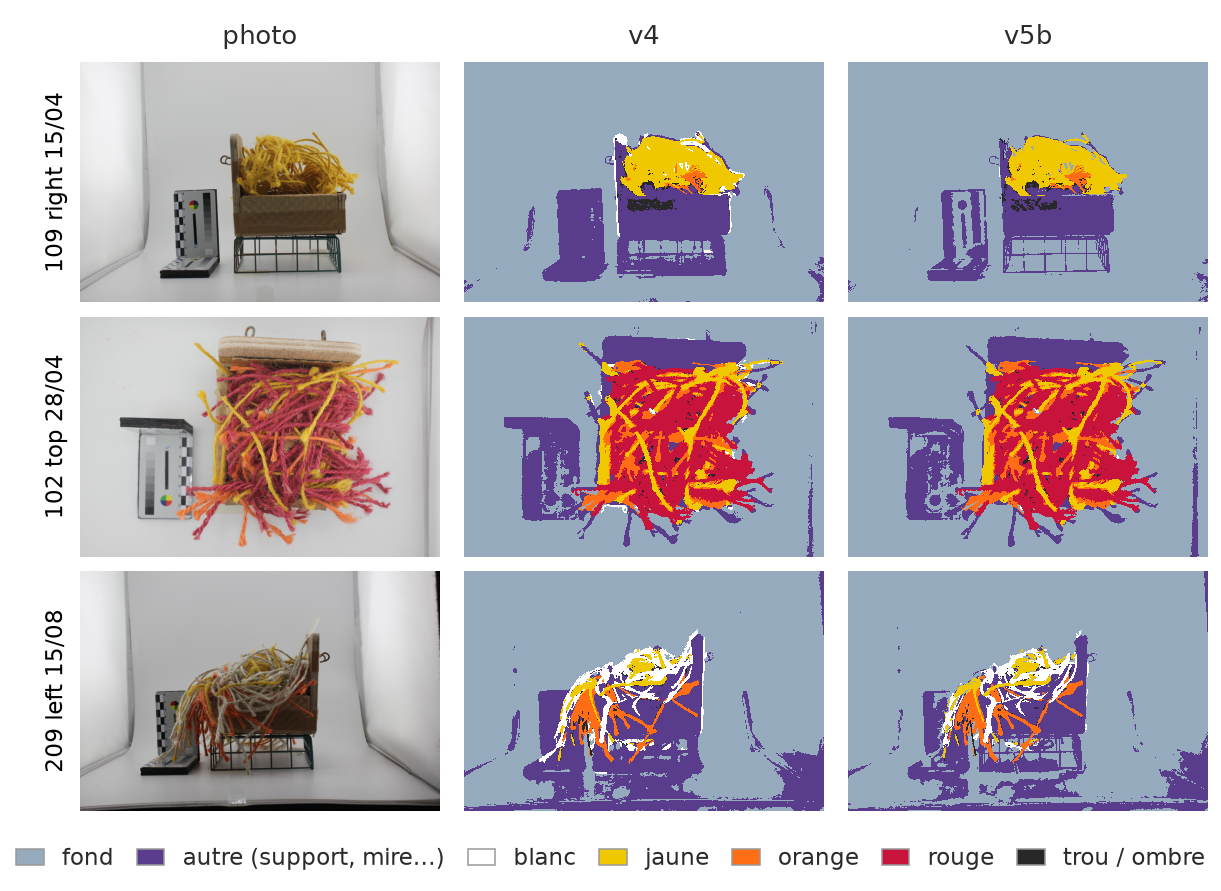
\includegraphics[width=0.82\textwidth]{figs/overview_allviews.png}
\caption{Images ajoutées après v3. En v4, aucune annotation ne portait sur ces images
(test de généralisation) : le nid 109, entièrement jaune, présente un liseré « blanc ».
En v5b, les exemples négatifs pris sur 109 et 102 le suppriment ; ces deux nids ne sont donc
plus des images de test indépendantes pour le blanc.}
\label{fig:overview-allviews}
\end{figure}

\section{Ce que chaque version corrige}

\begin{figure}[H]
\centering
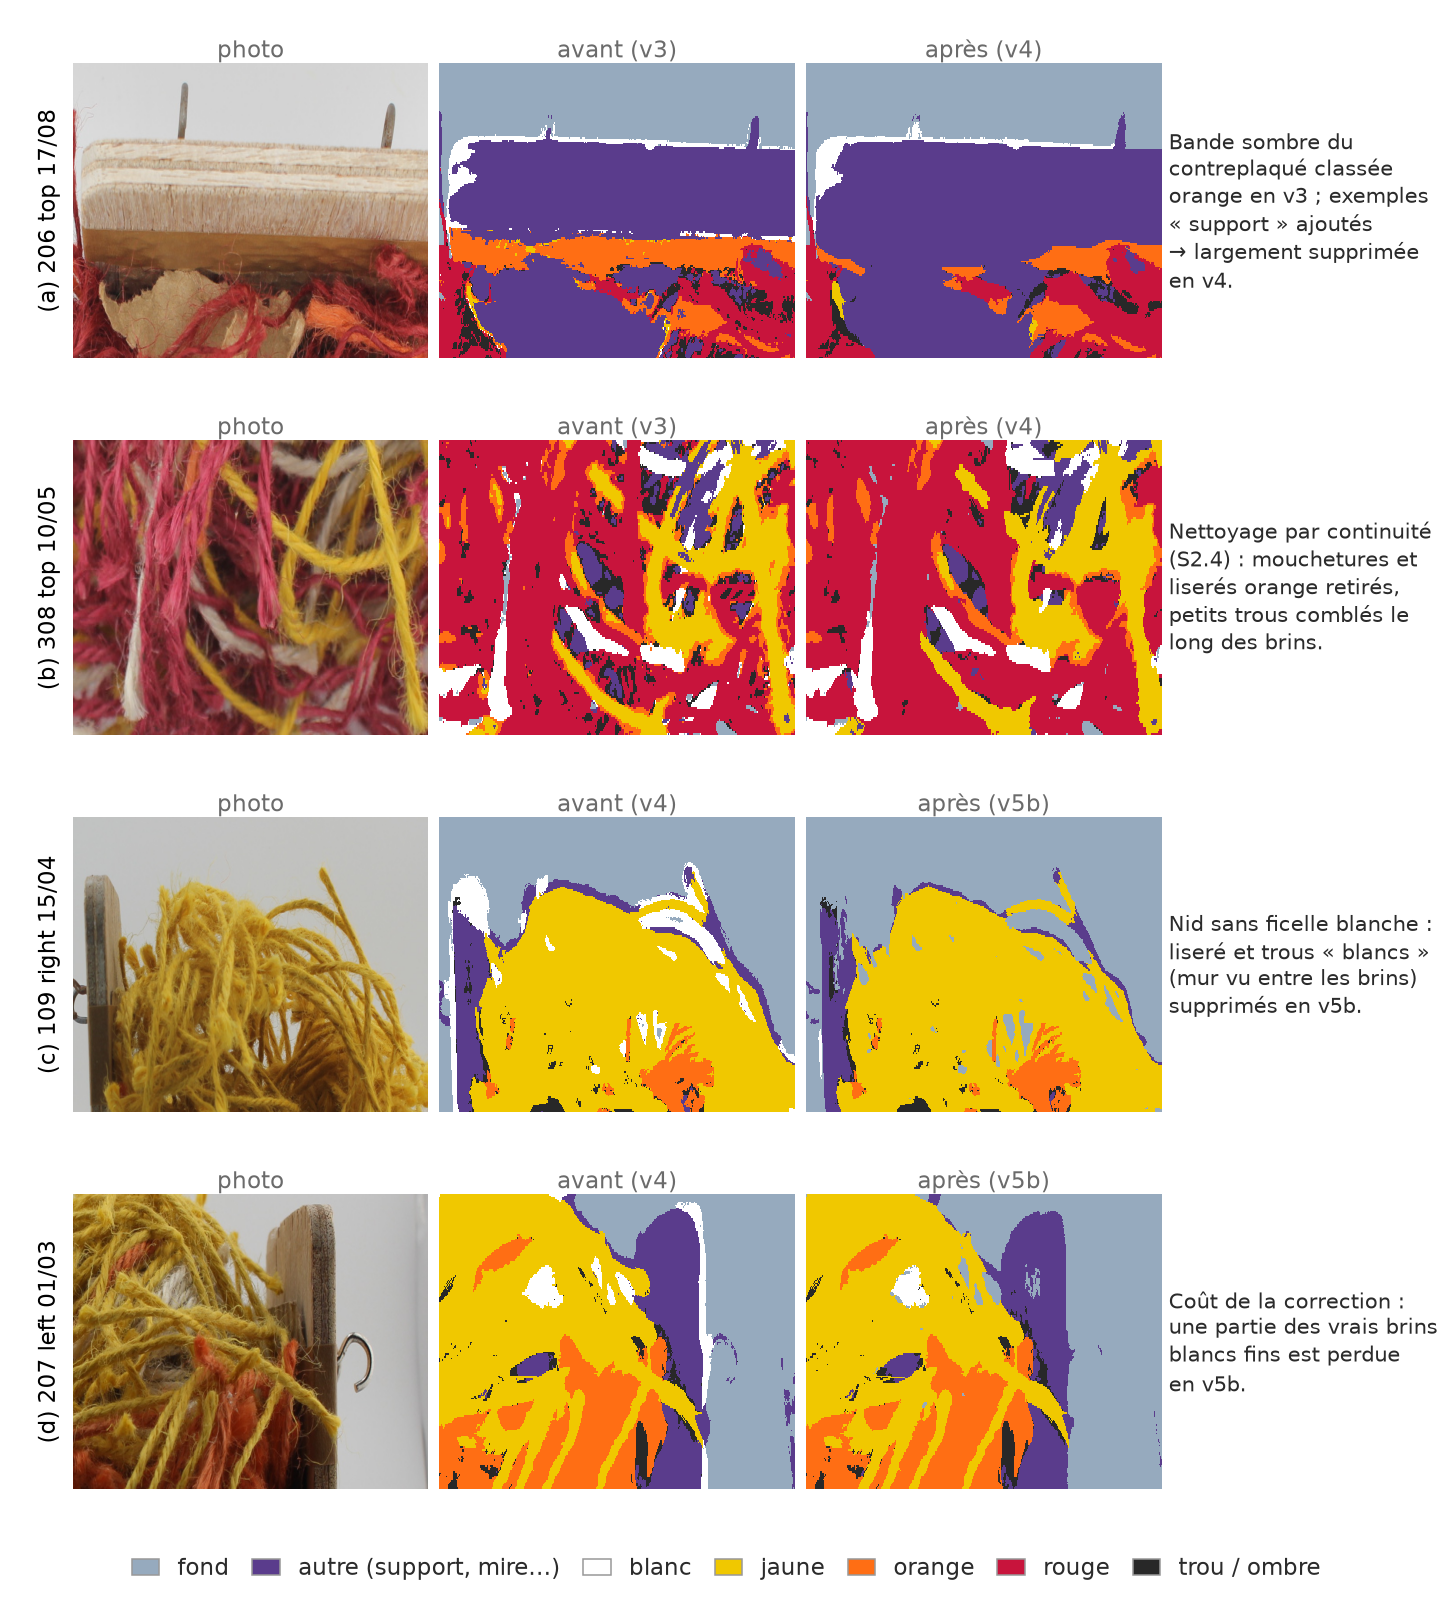
\includegraphics[width=\textwidth]{figs/zooms.png}
\caption{Zooms avant / après. (a) et (b) : passage de v3 à v4 ; (c) et (d) : passage de v4 à v5b.
La correction du faux blanc (c) a un coût : une partie des vrais brins blancs fins disparaît (d).}
\label{fig:zooms}
\end{figure}

Le tableau~\ref{tab:white} donne la part de blanc parmi les pixels de ficelle et la fraction de
pixels modifiés d'une version à l'autre. Sur les nids sans ficelle blanche (107, 206, 102 du 14/04,
109, 209 du 14/02), le blanc tombe à moins de 2\,\% en v5b, ce qui est le comportement attendu.
Sur les nids qui en contiennent réellement (207, 308, 209 du 15/08), il baisse aussi, de 4 à
10 points : v5b sous-estime probablement le blanc, v4 le surestimait.

\begin{table}[H]
\centering\small
\begin{tabular}{l rrr rr}
\toprule
 & \multicolumn{3}{c}{part de blanc (\% de la ficelle)} & \multicolumn{2}{c}{pixels modifiés (\%)} \\
\cmidrule(lr){2-4}\cmidrule(lr){5-6}
image & v3 & v4 & v5b & v3$\to$v4 & v4$\to$v5b \\
\midrule
107 top 26/05 & 0{,}9 & 0{,}1 & 0{,}0 & 2{,}2 & 1{,}2 \\
206 top 17/08 & 1{,}4 & 1{,}0 & 0{,}2 & 3{,}7 & 1{,}3 \\
207 front 01/03 & 26{,}5 & 26{,}0 & 21{,}7 & 2{,}8 & 5{,}4 \\
207 left 01/03 & 12{,}1 & 10{,}1 & 4{,}1 & 2{,}4 & 4{,}8 \\
207 right 01/03 & 25{,}5 & 23{,}6 & 15{,}2 & 2{,}4 & 5{,}3 \\
207 top 01/03 & 22{,}5 & 22{,}4 & 18{,}7 & 3{,}1 & 5{,}0 \\
208 top 29/08 & 84{,}0 & 84{,}4 & 83{,}5 & 3{,}5 & 5{,}2 \\
308 top 10/05 & 15{,}6 & 15{,}0 & 11{,}9 & 3{,}9 & 3{,}1 \\
\midrule \multicolumn{6}{l}{\textit{images ajoutées après v3 (pas de v3)}} \\
102 entrance 14/04 & -- & 6{,}5 & 0{,}0 & -- & 7{,}1 \\
102 entrance 28/04 & -- & 10{,}5 & 6{,}2 & -- & 4{,}5 \\
102 front 14/04 & -- & 2{,}2 & 0{,}0 & -- & 6{,}2 \\
102 front 28/04 & -- & 3{,}4 & 0{,}0 & -- & 5{,}0 \\
102 left 14/04 & -- & 3{,}4 & 0{,}0 & -- & 7{,}4 \\
102 left 28/04 & -- & 4{,}1 & 0{,}4 & -- & 4{,}5 \\
102 right 14/04 & -- & 4{,}7 & 0{,}1 & -- & 5{,}3 \\
102 right 28/04 & -- & 7{,}6 & 1{,}8 & -- & 5{,}5 \\
102 top 14/04 & -- & 6{,}4 & 0{,}2 & -- & 5{,}7 \\
102 top 28/04 & -- & 1{,}5 & 0{,}1 & -- & 2{,}7 \\
109 entrance 15/04 & -- & 7{,}8 & 1{,}7 & -- & 6{,}7 \\
109 front 15/04 & -- & 4{,}2 & 0{,}0 & -- & 6{,}4 \\
109 left 15/04 & -- & 5{,}9 & 0{,}1 & -- & 9{,}4 \\
109 right 15/04 & -- & 14{,}0 & 0{,}2 & -- & 6{,}2 \\
109 top 15/04 & -- & 8{,}7 & 0{,}1 & -- & 5{,}4 \\
209 entrance 14/02 & -- & 3{,}9 & 0{,}8 & -- & 5{,}5 \\
209 front 14/02 & -- & 4{,}0 & 0{,}0 & -- & 6{,}9 \\
209 front 15/08 & -- & 41{,}4 & 33{,}5 & -- & 7{,}9 \\
209 left 14/02 & -- & 5{,}0 & 0{,}3 & -- & 6{,}5 \\
209 left 15/08 & -- & 51{,}3 & 43{,}3 & -- & 6{,}9 \\
209 right 14/02 & -- & 3{,}2 & 0{,}0 & -- & 6{,}6 \\
209 right 15/08 & -- & 45{,}3 & 35{,}5 & -- & 7{,}6 \\
209 top 14/02 & -- & 4{,}3 & 0{,}6 & -- & 4{,}3 \\
209 top 15/08 & -- & 59{,}0 & 55{,}0 & -- & 7{,}4 \\
\bottomrule
\end{tabular}

\caption{Part de blanc (en \% des pixels de ficelle) et pixels modifiés entre versions. Le nid 207
figure une seule fois (mêmes photos dans les deux dossiers).}
\label{tab:white}
\end{table}

\section{Validation indépendante de v5b}

\paragraph{Protocole.} \valnpoints{} points ont été tirés au hasard, tous en dehors des rectangles
d'entraînement : 192 répartis uniformément dans la zone du nid (6 par image), pour estimer
l'exactitude sans biais, et 25 par classe prédite, pour que les classes rares (le blanc) aient assez de
points. Une annotatrice (M.\,D.) a classé chaque point sur une vignette de contexte et un zoom
centrés sur le point, sans voir la prédiction. Consigne : nommer la couleur dès qu'elle se
reconnaît, même à l'ombre ; « trou / ombre » seulement s'il n'y a aucun brin identifiable ;
« incertain » en cas de vrai doute (\valnunsure{} points, écartés). Fond et « autre » sont regroupés
en « non-ficelle », car les mesures n'utilisent pas la différence.

\paragraph{Résultats.} Exactitude globale \valacc{} [IC95 \valacclo--\valacchi] sur l'échantillon
uniforme ; \valaccstring{} sur les seuls points de ficelle. Quand le modèle et l'annotatrice voient
tous deux une couleur, elle est juste dans \valcolourok{} des cas ($n = \valncolour$).
Les erreurs viennent surtout d'ailleurs (tableaux~\ref{tab:scores} et~\ref{tab:confusion},
figure~\ref{fig:examples}) :
\begin{itemize}
\item \textbf{ficelle manquée} : \valmissed{} des vrais points de ficelle sont prédits non-ficelle,
  le blanc surtout (rappel 0,59). La moitié des cas sont des bords de brins, l'autre moitié des bouts
  effilochés isolés sur le fond ; 14 cas sur 15 sont perdus dès l'étage A ;
\item \textbf{jaune à l'ombre pris pour de l'orange} : la précision de l'orange n'est que de 0,62 ;
  cette confusion crée des contacts jaune--orange fictifs et peut surestimer le mélange ;
\item \textbf{classe « trou / ombre » trop large} : elle contient surtout de la ficelle dont
  la couleur reste reconnaissable à l'œil. Ces pixels sont perdus mais non mal étiquetés
  (\vallostshadow{} des vraies couleurs).
\end{itemize}

\begin{table}[H]
\centering\small
\begin{tabular}{l rr rr}
\toprule
classe & \multicolumn{2}{c}{précision (tous les points)} & \multicolumn{2}{c}{rappel (uniforme)} \\
\cmidrule(lr){2-3}\cmidrule(lr){4-5}
 & valeur [IC95] & $n$ & valeur [IC95] & $n$ \\
\midrule
non-ficelle & 0{,}85 [0{,}78--0{,}90] & 145 & 0{,}96 [0{,}89--0{,}99] & 79 \\
blanc & 0{,}94 [0{,}80--0{,}98] & 33 & 0{,}59 [0{,}36--0{,}78] & 17 \\
jaune & 0{,}95 [0{,}87--0{,}98] & 66 & 0{,}80 [0{,}67--0{,}89] & 50 \\
orange & 0{,}62 [0{,}47--0{,}75] & 42 & 0{,}72 [0{,}49--0{,}88] & 18 \\
rouge & 0{,}88 [0{,}73--0{,}95] & 34 & 0{,}80 [0{,}49--0{,}94] & 10 \\
trou/ombre & 0{,}29 [0{,}15--0{,}47] & 28 & 0{,}00 [-0{,}00--0{,}28] & 10 \\
\bottomrule
\end{tabular}

\caption{Précision (« quand le modèle dit X, est-ce X ? ») sur tous les points prédits X ;
rappel (« un vrai X est-il vu comme X ? ») sur l'échantillon uniforme. Intervalles de Wilson à 95\,\%.}
\label{tab:scores}
\end{table}

\begin{table}[H]
\centering\small
\begin{tabular}{lrrrrrr}
\toprule
vérité $\downarrow$ \quad prédiction $\rightarrow$ & non-ficelle & blanc & jaune & orange & rouge & trou/ombre \\
\midrule
non-ficelle & \textbf{76} & 0 & 1 & 1 & 0 & 1 \\
blanc & 5 & \textbf{10} & 1 & 1 & 0 & 0 \\
jaune & 3 & 0 & \textbf{40} & 5 & 0 & 2 \\
orange & 5 & 0 & 0 & \textbf{13} & 0 & 0 \\
rouge & 1 & 0 & 0 & 0 & \textbf{8} & 1 \\
trou/ombre & 5 & 0 & 1 & 2 & 2 & \textbf{0} \\
\bottomrule
\end{tabular}

\caption{Matrice de confusion, échantillon uniforme (\valnuniform{} points, incertains écartés).
En gras, les bonnes réponses.}
\label{tab:confusion}
\end{table}

\begin{figure}[H]
\centering
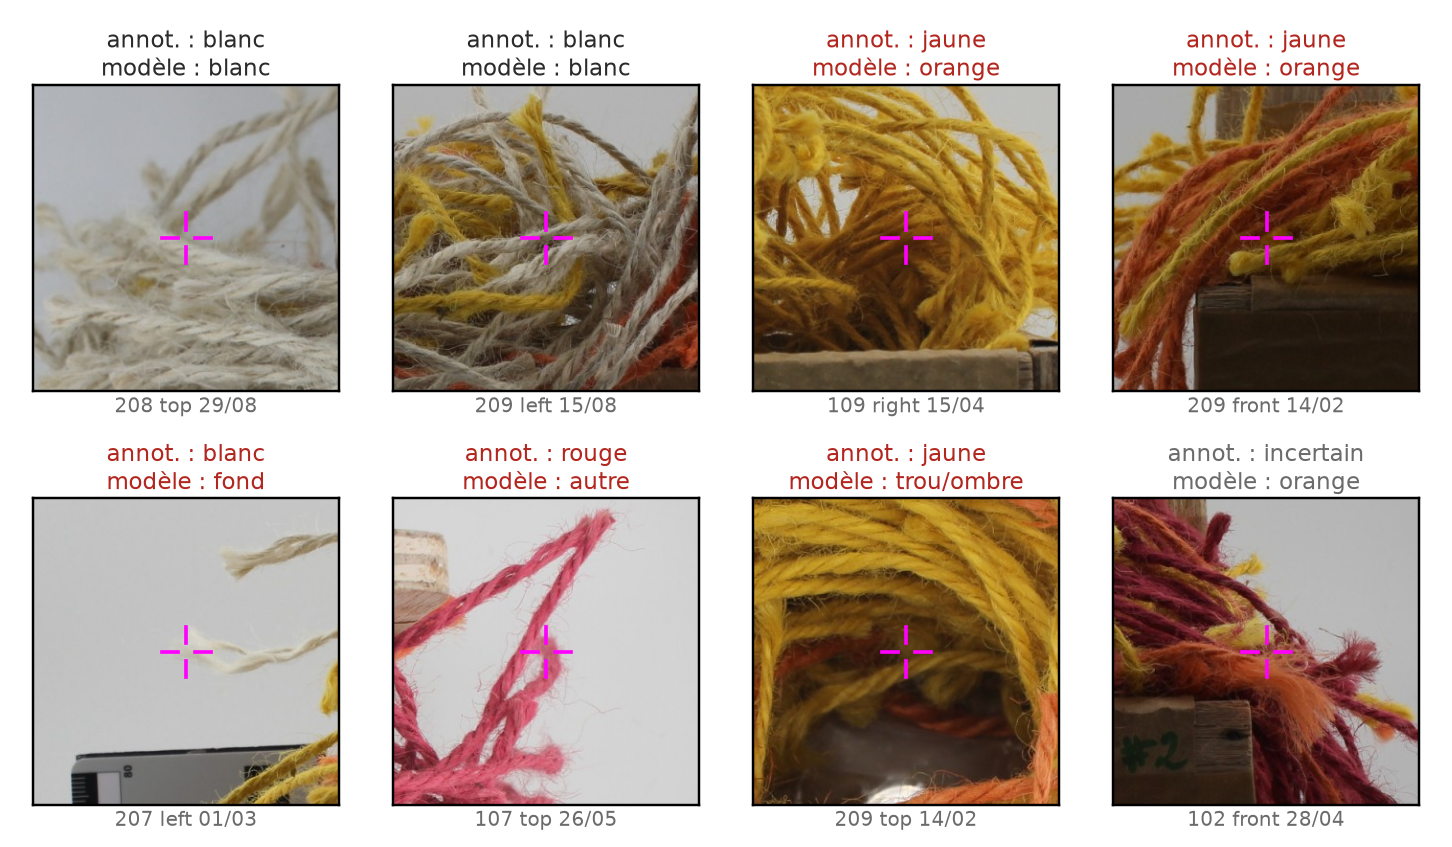
\includegraphics[width=\textwidth]{figs/validation_examples.png}
\caption{Exemples de points de validation (vignette de contexte, le viseur marque le point).
En haut à gauche, deux réussites sur le blanc ; en rouge, les erreurs typiques : jaune à l'ombre
classé orange, bouts fins sur le fond manqués, jaune assombri classé « trou / ombre ».
En bas à droite, un point jugé incertain (duvet orange devant des brins rouges).}
\label{fig:examples}
\end{figure}

\section{Limites et suite}

\begin{itemize}
\item Les rectangles d'entraînement ont été tracés par un annotateur non expert, et les filtres de
  couleur définissent en partie ce qu'est « du jaune » : d'où l'importance de la validation à
  l'aveugle, qui ne dépend pas de ces choix.
\item Une seule annotatrice : l'accord entre deux annotateurs n'est pas encore mesuré.
\item Le blanc reste la classe la moins fiable ; la conclusion sur le mélange et la stratification
  est peu sensible au choix v4 / v5b (écarts d'indice $\leq 0{,}1$).
\item Pistes, à revalider sur les mêmes \valnpoints{} points : étage A à pleine résolution pour les
  bouts fins ; couleur indépendante de la luminance pour séparer jaune sombre et orange ;
  seuil d'ombre plus bas.
\end{itemize}

\end{document}
